  
\documentclass[titlepage]{article}
\usepackage[utf8]{inputenc}
\usepackage{amsmath}
\usepackage{tcolorbox}
\usepackage{amssymb}
\usepackage{amsthm}
\usepackage{empheq}
\usepackage{xcolor}
\usepackage{float}
\usepackage[
top    = 2.50cm,
bottom = 2.50cm,
left   = 2.75cm,
right  = 2.75cm]{geometry}
\usepackage{fancyhdr}
\pagestyle{fancy}
\lhead{Analysis 2}
\rhead{EPFL/Alp Ozen}

\newtheorem{remark}{Remark}[section]
\newtheorem{theorem}{Theorem}[section]
\newtheorem{prop}{[Proposition]}
\newtheorem{definition}{Definition}
\newtheorem{question}{Question}

\newcommand{\interior}[1]{%
  {\kern0pt#1}^{\mathrm{o}}%
}
\newcommand{\Rn}{\mathbb{R}^n}
\newcommand{\Rm}{\mathbb{R}^m}
\newcommand{\R}{\mathbb{R}}

\title{\textbf{Digital System Design - Theo Kluter}}
\author{Alp Ozen}
\date{Spring 2019}
\newtheorem{example}{Example}[section]
\newtheorem{axiom}{Axiom}
\newtheorem{cor}{Corollary}

\begin{document}

\maketitle
\tableofcontents
\clearpage

\section{Course Part 1}

\subsection{Boolean algebra}

We begin by listing basics of Boolean algebra:
We also note that in these notes $\land \equiv \cdot$ and $\lor \equiv +$

\begin{figure}[H]
    \centering
    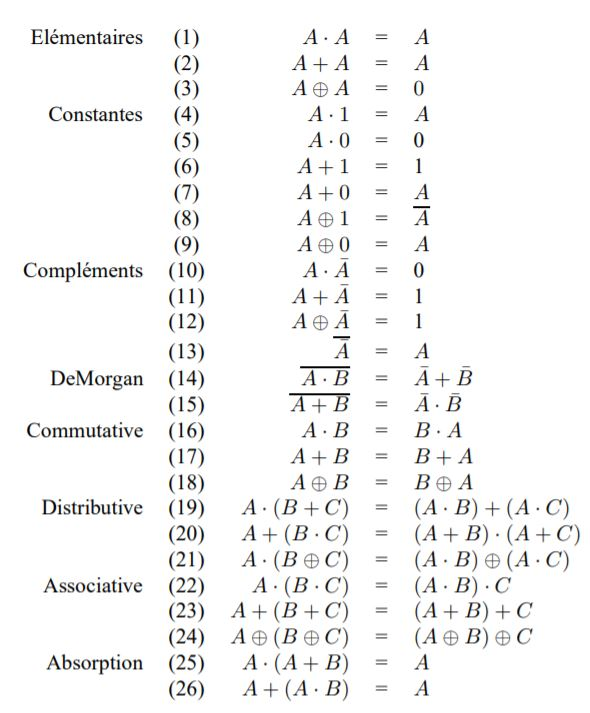
\includegraphics{src/bool.JPG}
    \caption{Boolean algebra}
    \label{Boolean algebra}
\end{figure}

When trying to decode a truth table, it is practical to use a Karnaugh diagram, find the 'dont-care' terms and arrive at an expression. Note that each 'block' will produce one expression. 

\begin{figure}[H]
    \centering
    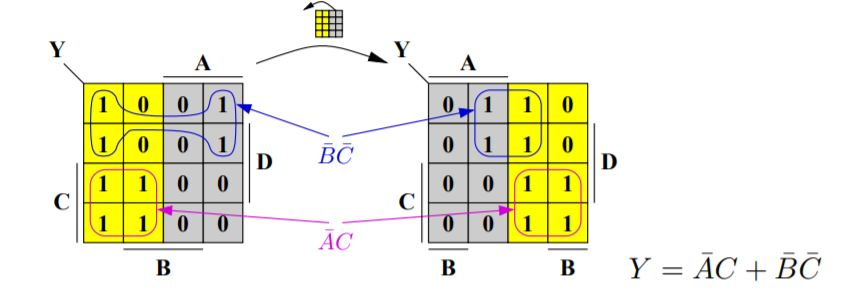
\includegraphics{src/bool2.JPG}
    \caption{Karnaugh diagram}
    \label{fig:my_label}
\end{figure}

\subsection{Latches}
How do we go about creating a circuit that is able to memorize? How about connecting an output as an input? The simplest example of this is the "SR" aka. "Set-Reset" latch as below:


\begin{figure}[H]
    \centering
    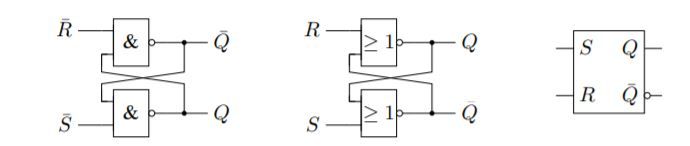
\includegraphics[scale = 0.7]{src/bool3.JPG}
    \caption{SR Latch}
    \label{fig:my_label}
\end{figure}

We note that if we are to add two inverters to the above 3 circuits(which are all equivalent), we will obtain a circuit with a Set priority. That is, upon pressing button 1, light 1 lights up and etc. The earlier version without inverter is the Reset priority version where upon pressing button 1, light 2 lights up. 
\\

Expanding on the SR latch, we have the D-latch. This latch has two inputs, an enable button and an input button. When enable is on(set to 1), our latch enters transparent mode and the output takes the value of D our input. When enable is off, the latch will remember the last value of D and become disactivated. 


\end{document} 
